%%%%%%%%%%%%%%%%%%%%%%%%%%%%%%%%%%%%%%%%%
% Beamer Presentation
% LaTeX Template
% Version 1.0 (10/11/12)
%
% This template has been downloaded from:
% http://www.LaTeXTemplates.com
%
% License:
% CC BY-NC-SA 3.0 (http://creativecommons.org/licenses/by-nc-sa/3.0/)
%
%%%%%%%%%%%%%%%%%%%%%%%%%%%%%%%%%%%%%%%%%

%----------------------------------------------------------------------------------------
%  PACKAGES AND THEMES
%----------------------------------------------------------------------------------------

\documentclass[table]{beamer}\usepackage[]{graphicx}\usepackage[]{color}
%% maxwidth is the original width if it is less than linewidth
%% otherwise use linewidth (to make sure the graphics do not exceed the margin)
\makeatletter
\def\maxwidth{ %
  \ifdim\Gin@nat@width>\linewidth
    \linewidth
  \else
    \Gin@nat@width
  \fi
}
\makeatother

\definecolor{fgcolor}{rgb}{0.345, 0.345, 0.345}
\newcommand{\hlnum}[1]{\textcolor[rgb]{0.686,0.059,0.569}{#1}}%
\newcommand{\hlstr}[1]{\textcolor[rgb]{0.192,0.494,0.8}{#1}}%
\newcommand{\hlcom}[1]{\textcolor[rgb]{0.678,0.584,0.686}{\textit{#1}}}%
\newcommand{\hlopt}[1]{\textcolor[rgb]{0,0,0}{#1}}%
\newcommand{\hlstd}[1]{\textcolor[rgb]{0.345,0.345,0.345}{#1}}%
\newcommand{\hlkwa}[1]{\textcolor[rgb]{0.161,0.373,0.58}{\textbf{#1}}}%
\newcommand{\hlkwb}[1]{\textcolor[rgb]{0.69,0.353,0.396}{#1}}%
\newcommand{\hlkwc}[1]{\textcolor[rgb]{0.333,0.667,0.333}{#1}}%
\newcommand{\hlkwd}[1]{\textcolor[rgb]{0.737,0.353,0.396}{\textbf{#1}}}%

\usepackage{framed}
\makeatletter
\newenvironment{kframe}{%
 \def\at@end@of@kframe{}%
 \ifinner\ifhmode%
  \def\at@end@of@kframe{\end{minipage}}%
  \begin{minipage}{\columnwidth}%
 \fi\fi%
 \def\FrameCommand##1{\hskip\@totalleftmargin \hskip-\fboxsep
 \colorbox{shadecolor}{##1}\hskip-\fboxsep
     % There is no \\@totalrightmargin, so:
     \hskip-\linewidth \hskip-\@totalleftmargin \hskip\columnwidth}%
 \MakeFramed {\advance\hsize-\width
   \@totalleftmargin\z@ \linewidth\hsize
   \@setminipage}}%
 {\par\unskip\endMakeFramed%
 \at@end@of@kframe}
\makeatother

\definecolor{shadecolor}{rgb}{.97, .97, .97}
\definecolor{messagecolor}{rgb}{0, 0, 0}
\definecolor{warningcolor}{rgb}{1, 0, 1}
\definecolor{errorcolor}{rgb}{1, 0, 0}
\newenvironment{knitrout}{}{} % an empty environment to be redefined in TeX

\usepackage{alltt}

% The Beamer class comes with a number of default slide themes
% which change the colors and layouts of slides. Below this is a list
% of all the themes, uncomment each in turn to see what they look like.

%\usetheme{default}
%\usetheme{AnnArbor}
%\usetheme{Antibes}
%\usetheme{Bergen}
%\usetheme{Berkeley}
%\usetheme{Berlin}
%\usetheme{Boadilla}
\usetheme{CambridgeUS}
%\usetheme{Copenhagen}
%\usetheme{Darmstadt}
%\usetheme{Dresden}
%\usetheme{Frankfurt}
%\usetheme{Goettingen}
%\usetheme{Hannover}
%\usetheme{Ilmenau}
%\usetheme{JuanLesPins}
%\usetheme{Luebeck}
%\usetheme{Madrid}
%\usetheme{Malmoe}
%\usetheme{Marburg}
%\usetheme{Montpellier}
%\usetheme{PaloAlto}
%\usetheme{Pittsburgh}
%\usetheme{Rochester}
%\usetheme{Singapore}
%\usetheme{Szeged}
%\usetheme{Warsaw}

% As well as themes, the Beamer class has a number of color themes
% for any slide theme. Uncomment each of these in turn to see how it
% changes the colors of your current slide theme.

%\usecolortheme{albatross}
\usecolortheme{beaver}
%\usecolortheme{beetle}
%\usecolortheme{crane}
%\usecolortheme{dolphin}
%\usecolortheme{dove}
%\usecolortheme{fly}
%\usecolortheme{lily}
%\usecolortheme{orchid}
%\usecolortheme{rose}
%\usecolortheme{seagull}
%\usecolortheme{seahorse}
%\usecolortheme{whale}
%\usecolortheme{wolverine}

%\setbeamertemplate{footline} % To remove the footer line in all slides uncomment this line
%\setbeamertemplate{footline}[page number] % To replace the footer line in all slides with a simple slide count uncomment this line

%\setbeamertemplate{navigation symbols}{} % To remove the navigation symbols from the bottom of all slides uncomment this line


\usepackage{graphicx} % Allows including images
\usepackage{booktabs} % Allows the use of \toprule, \midrule and \bottomrule in tables
\usepackage{xcolor}
\usepackage{tabu}  % Even fancier than tabulary
\usepackage{multirow}
\usepackage{textcomp} %  Text style for code snippets inline in text:
\newcommand{\codeInline}[1]{\texttt{#1}}
%\usepackage{Sweave}

%----------------------------------------------------------------------------------------
%	TITLE PAGE
%----------------------------------------------------------------------------------------

\title[Group3:Data Analysis]{Group 3: Data Analysis} % The short title appears at the bottom of every slide, the full title is only on the title page

\author[Emily, Liza, Nick and Yiding]{Nick Cummings, Liza Nicoll, Emily Ramos, and Yiding Zhang} % Your name
\institute[UMASS] % Your institution as it will appear on the bottom of every slide, may be shorthand to save space
{
University of Massachusetts, Amherst \\ % Your institution for the title page
\medskip
%\textit{} % Your email address
}
\date{\today} % Date, can be changed to a custom date
\IfFileExists{upquote.sty}{\usepackage{upquote}}{}

\begin{document}
%\SweaveOpts{concordance=TRUE}

\begin{frame}
\titlepage % Print the title page as the first slide
\end{frame}

\begin{frame}
\frametitle{Overview} % Table of contents slide, comment this block out to remove it
\tableofcontents % Throughout your presentation, if you choose to use \section{} and \subsection{} commands, these will automatically be printed on this slide as an overview of your presentation
\end{frame}

%----------------------------------------------------------------------------------------
%	PRESENTATION SLIDES
%----------------------------------------------------------------------------------------

%------------------------------------------------
\section{Group Analysis} % Sections can be created in order to organize your presentation into discrete blocks, all sections and subsections are automatically printed in the table of contents as an overview of the talk
%------------------------------------------------

\subsection{Introduction} % A subsection can be created just before a set of slides with a common theme to further break down your presentation into chunks

\begin{frame}{Introduction}



\begin{columns}[c] % contents are top vertically aligned
\begin{column}[c]{6cm} % each column can also be its own environment
{\fontsize{0.3cm}{1em}\selectfont
\begin{itemize}
  \item The dataset, ``Exploring Relationships in Body Dimensions", contains 25 variables: 21 body dimension measurements as well as age, weight, height, and gender for 507 physically active, young individuals.
  \item Of the body dimension measurements, 9 were skeletal/diameter measurements and 12 were girth/circumference measurements.
  \item Of the 507 individual observations, there are 247 men and 260 women.
  \item No missing values. Measurements made with metric scale.
\end{itemize}
}
\end{column}

\begin{column}[c]{6cm} 
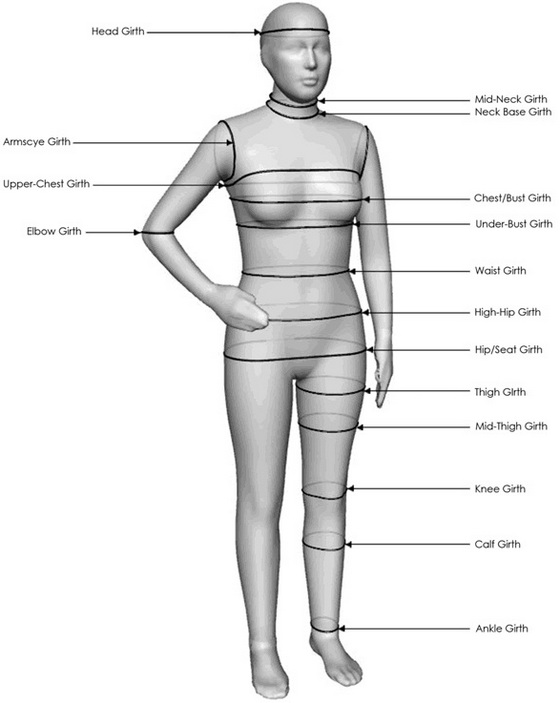
\includegraphics[width=\textwidth]{body}
\end{column}
\end{columns}

\end{frame}

%------------------------------------------------

\subsection{Description of Variables}

%------------------------------------------------
\begin{frame}{Description of Variables}
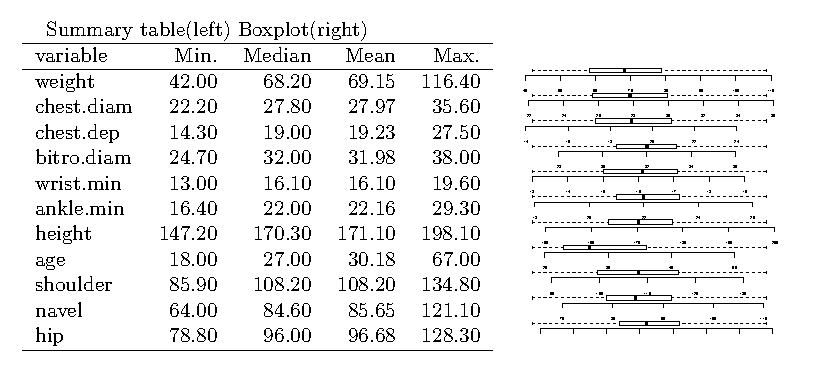
\includegraphics[width=\textwidth]{summary_table}

\end{frame}


%------------------------------------------------

\subsection{Outcome of Interest}

%------------------------------------------------

\begin{frame}{Outcome of Interest: Weight}

\begin{columns}[c] % contents are top vertically aligned
\begin{column}[c]{5cm} % each column can also be its own environment
{\fontsize{0.275cm}{1em}\selectfont

Applications of Data: 
\begin {itemize}
  \item investigate correspondence of frame size, girths, and weight of young, athletic people
  \item  estimate ideal weight
  \item  inform predictions of lean/fat body compositions
  \item  identify gender in forensic science
  \item  design appropriate clothing (law enforcement/military) 
\end{itemize}

Note: Outliers in the distribution of weight may be present because some of the individuals had unusually high muscle mass due to their high level of physical fitness.

}
\end{column}

\begin{column}[c]{7cm} 
\begin{knitrout}
\definecolor{shadecolor}{rgb}{0.969, 0.969, 0.969}\color{fgcolor}
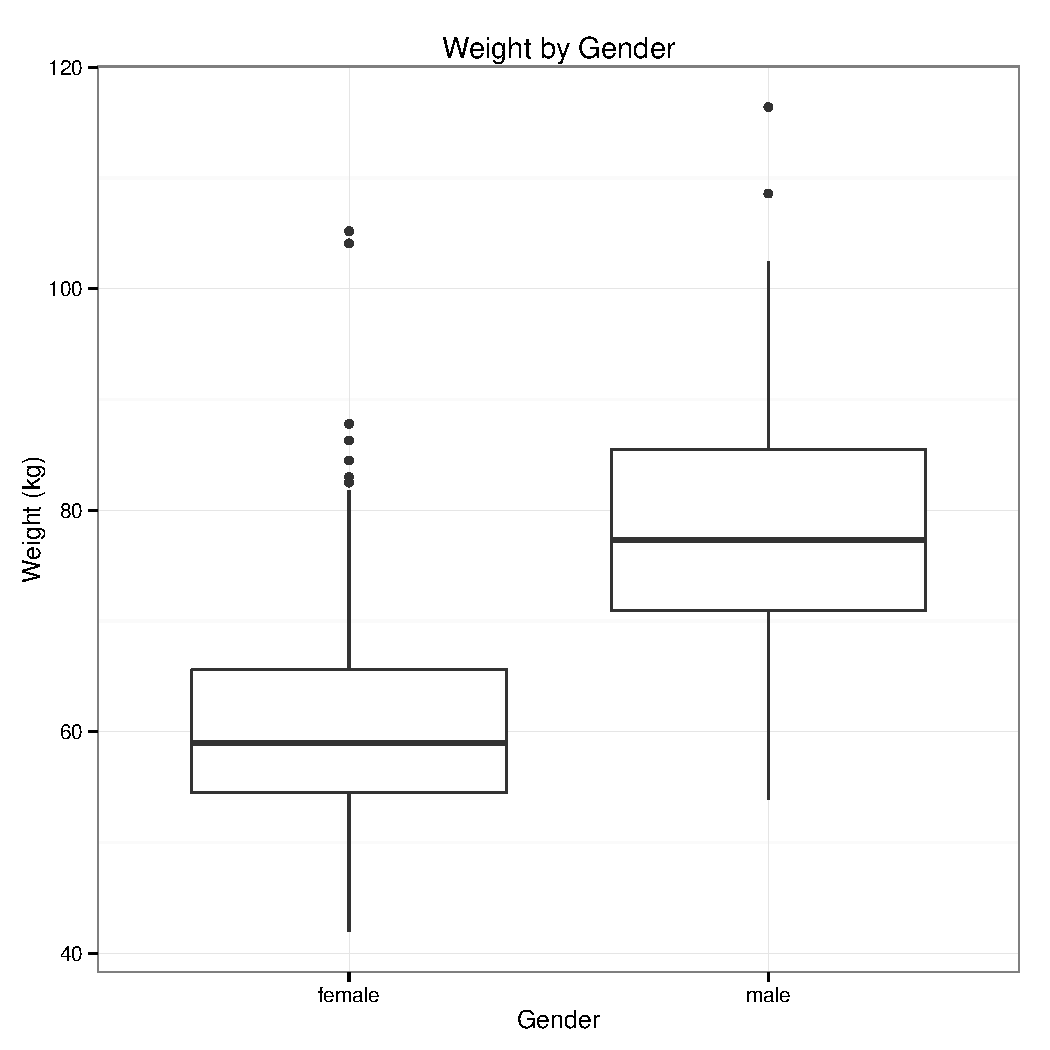
\includegraphics[width=\maxwidth]{figure/weight_plot} 

\end{knitrout}

\end{column}
\end{columns}
\end{frame}

%------------------------------------------------

\subsection{Initial Model}

%------------------------------------------------

\begin{frame}{Multiple Linear Regression Model}

\begin{block}{Initial Model}
\begin{eqnarray*}
\text{weight}_i &=& \beta_0 + \beta_1 \text{chest.diam}_{i} + \beta_2 \text{chest.dep}_{i} + \beta_3 \text{bitro.diam}_{i} \\
&& + \beta_4 \text{wrist.min}_{i} + \beta_5 \text{ankle.min}_{i} + \beta_6 \text{height}_{i}
\end{eqnarray*}
\end{block}

\\

\texbf{R Output:}\\

\\

{\fontsize{0.275cm}{1em}\selectfont 
\begin{tabular}{|r|r|r|r|r|r|r|r|}
\hline
    (Intercept) & chest.diam & chest.dep & bitro.diam & wrist.min & ankle.min & height & R^2 \\ \hline
   -109.89 & 1.34  & 1.54 & 1.20  & 1.11 & 1.15 & 0.18 & 0.8882 \\ \hline
\end{tabular}

\begin{itemize}
  \item This model was chosen by the authors of the dataset based on the idea that these measurements remain constant after physical maturation.
  \item It seems that, in our model, chest depth has the largest impact on weight.
  \item Model seems like a good fit, but can we find a better one?
\end{itemize}

}
\end{frame}


%------------------------------------------------

\section{Individual Analysis}

%------------------------------------------------

\subsection{Model Diagnostics}

%------------------------------------------------

\begin{frame}{Model Diagnostics (Nick)}
Model Diagnostics are important to fitting an appropriate model
\begin{itemize}
  \item Outliers: extreme points that are distant form the other observations, measured by residuals
  \item Leverage: an extreme point, measured by the hat matrix. An ``outlier on the X axis"
  \item Influential Points: points that have a large effect on the slope of the model
  \item Influence = Leverage + ``Outlyingness"
\end{itemize}
\end{frame}

%------------------------------------------------

\begin{frame}{Outliers (Nick)}
  \begin{columns}[t] % vertically aligned
  \begin{column}[c]{6cm}

\begin{itemize}
  \item Assumption violations can lead to biased or faulty results
  \item Outliers are commonly measurement errors, or are points indicative of a population that has a heavy tailed distribution
  \item Outliers are present in the model (points 124, 359, 474) 
\end{itemize}

  \end{column}
  \begin{column}[c]{4.5cm}
  
\begin{knitrout}
\definecolor{shadecolor}{rgb}{0.969, 0.969, 0.969}\color{fgcolor}
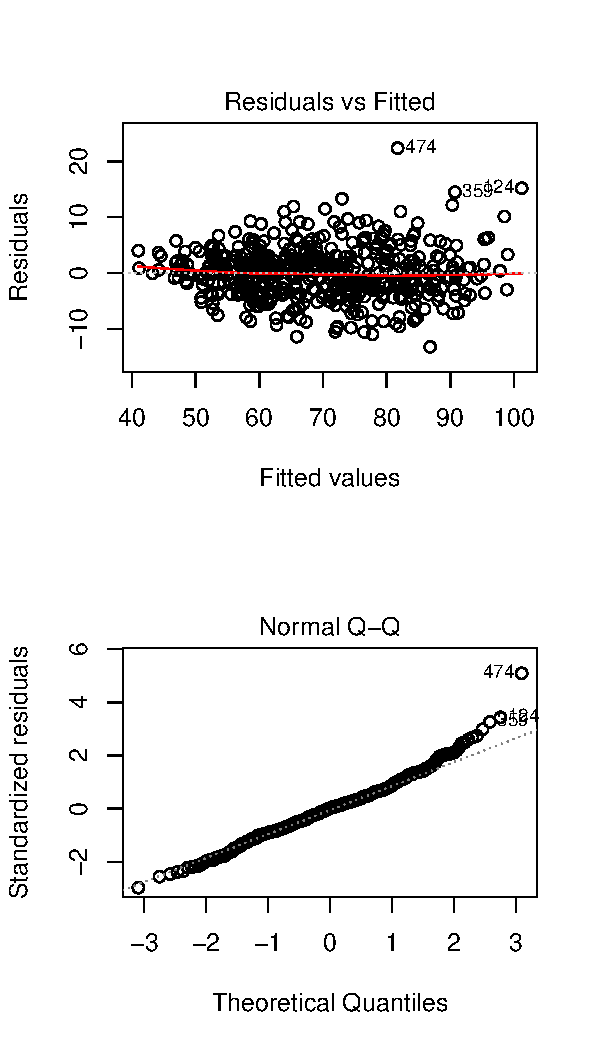
\includegraphics[width=\maxwidth]{figure/residual_plots} 

\end{knitrout}


  \end{column}
  \end{columns}

\end{frame}
%------------------------------------------------

\begin{frame} {Leverage (Nick)} %make and interpret leverage plots

A "rule of thumb" is that leverages of more than $\dfrac{2p}{n}$ or $\dfrac{3p}{n}$ should be looked at more closely.  Points of concern are located above the red line. 

\begin{knitrout}
\definecolor{shadecolor}{rgb}{0.969, 0.969, 0.969}\color{fgcolor}
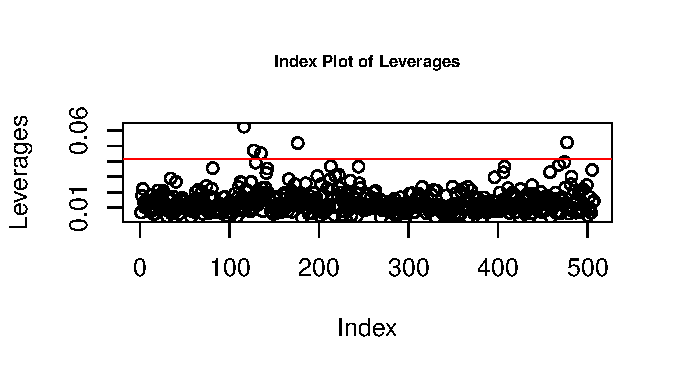
\includegraphics[width=\maxwidth]{figure/leverage} 

\end{knitrout}



\end{frame}

%-----------------------------------------------------

\begin{frame}{Influence (Nick)}  

{\fontsize{0.3cm}{1em}\selectfont
An \textbf{influential point} is one whose removal from the dataset causes a drastic change in the fit.  An influential point will either be an outlier in the data, will have high leverage, or will have both.}




\begin{center}
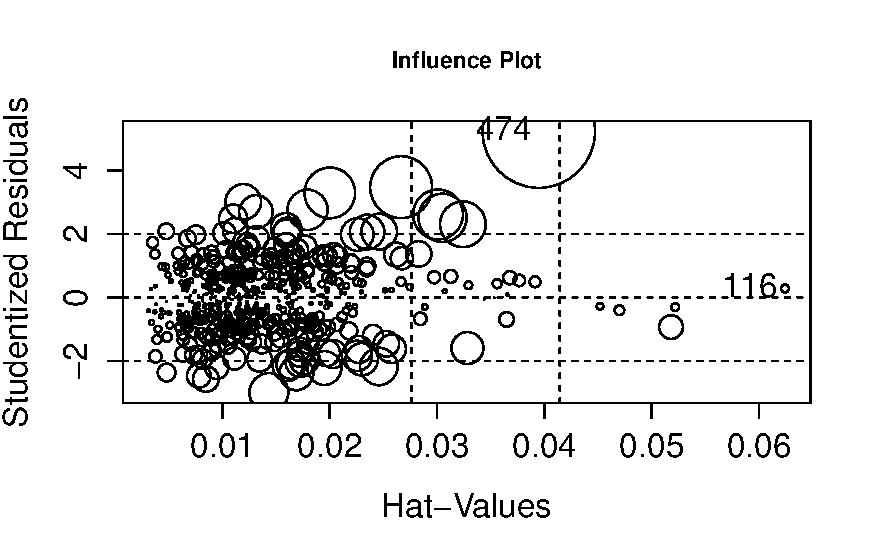
\includegraphics[width=0.8\textwidth]{influence}
\end{center}

\end{frame}
%------------------------------------------------

\begin{frame} {Cook's Distance (Nick)}
\begin{columns}[t]
\begin{column}[c]{5cm}

\begin{itemize}
  \item We can look at leverage, outlyingness, and influence altogether
  \item The Cook's Distance plot shows the values of these problematic points
  \item When we remove these points, does the model improve much?
\end{itemize}
\end{column}

\begin{column}[c]{7cm}

\begin{knitrout}
\definecolor{shadecolor}{rgb}{0.969, 0.969, 0.969}\color{fgcolor}
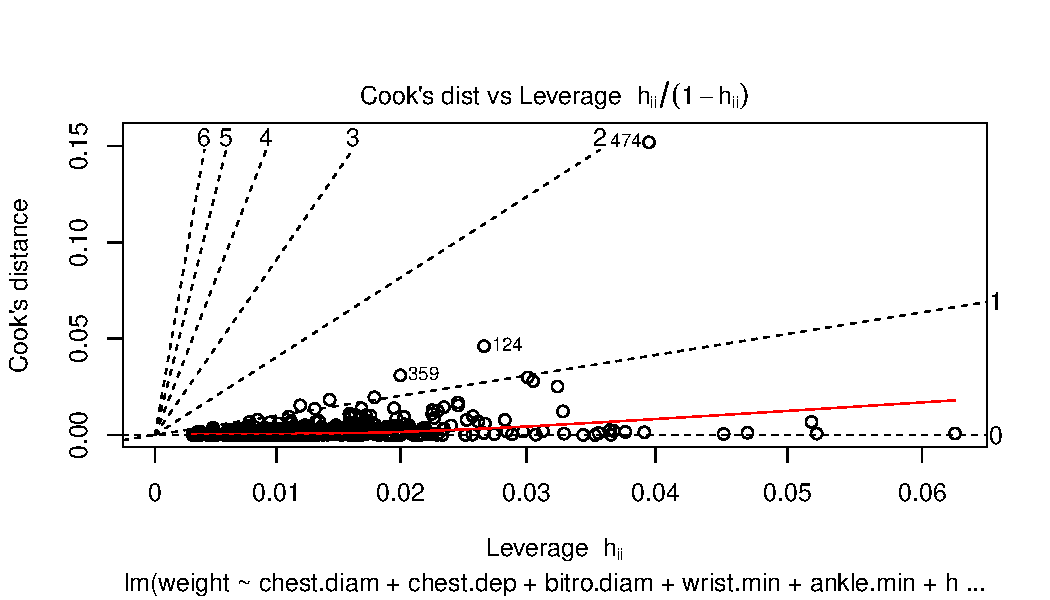
\includegraphics[width=\maxwidth]{figure/unnamed-chunk-1} 

\end{knitrout}

\end{column}
\end{columns}
\end{frame}


%------------------------------------------------

\begin{frame} {Better Fit? (Nick)} 

Initial Model: \\

{\fontsize{0.275cm}{1em}\selectfont 
\begin{tabular}{|r|r|r|r|r|r|r|r|}
\hline
    (Inter.) & chest.diam & chest.dep & bitro.diam & wrist.min & ankle.min & height & Adj. $R^2$ \\ \hline
   -109.89 & 1.34  & 1.54 & 1.20  & 1.11 & 1.15 & 0.18 & 0.887 \\ \hline
   
\end{tabular}
}

\linebreak[4]

New model with influential points removed:\\

{\fontsize{0.275cm}{1em}\selectfont 
\begin{tabular}{|r|r|r|r|r|r|r|r|}
\hline
    (Inter.) & chest.diam & chest.dep & bitro.diam & wrist.min & ankle.min & height & Adj. $R^2$ \\ \hline
   -109.11 & 1.38  & 1.55 & 1.10  & 0.97 & 1.17 & 0.19 & 0.891 \\ \hline

\end{tabular}

}

\begin{center}
\includegraphics[width=0.7\textwidth]{outlier}
\end{center}

\end{frame}

%------------------------------------------------

\subsection{Model Selection}

%------------------------------------------------
\begin{frame}{Model Selection Criteria and Methods (Emily)}

\begin{center}
\textbf{Goal:} Find the ``best" method for model selection.\\
\end{center}

\begin{columns}[c] % contents are top vertically aligned
\begin{column}[c]{5cm} % each column can also be its own environment
The methods used to create ten different models were:
\begin{itemize}
\item include all variables (1)\\
\item suggested by paper (2)\\
\item my selection (1)\\
\item stepAIC (1) \\
\item leaps (2) \\
\item combinations of R functions and human intuition (3).  \\
\end{itemize}

\end{column}

\begin{column}[c]{7cm} 

These models were compared using: \\
\begin{itemize}
\item AIC/ BIC: measure goodness-of-fit through residual sum of squares and penalizes for adding more predictors; the smaller the better.\\
\item Adjusted $R^2$: adjusts $R^2$ so that the model is penalized for adding more predictors; the larger the better. \\
\item PRESS is a summary measure focused on prediction; the smaller the better.\\
\end{itemize}
\end{column}
\end{columns}
\end{frame}

%------------------------------------------------
\begin{frame}{My Selection (Emily)}

\begin{columns}[t] % contents are top vertically aligned
\begin{column}[T]{5cm} % each column can also be its own environment
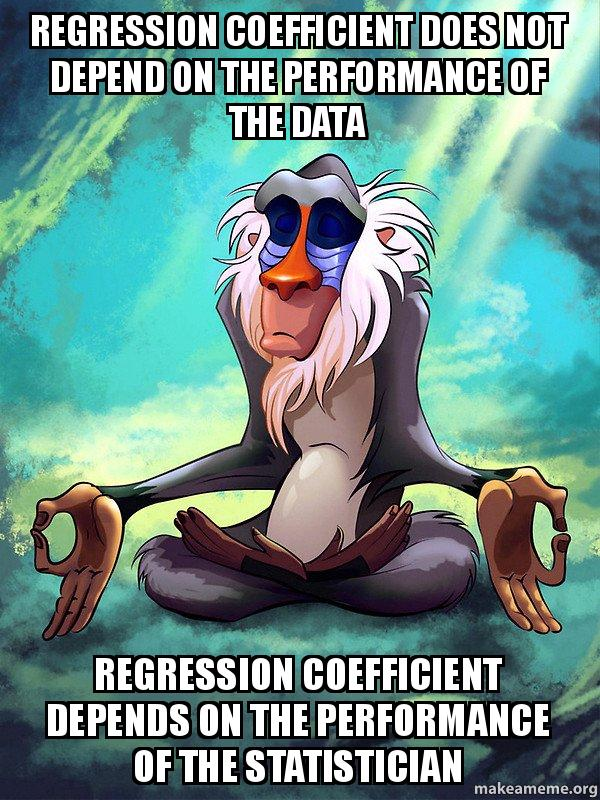
\includegraphics[width=\textwidth]{rafiki}
\end{column}

\begin{column}[T]{7cm} 

\begin{itemize}
\item \textbf{Predictors needed:} age, height and gender (since these contribute significantly to weight) \\

\item \textbf{Predictors we will allow:} the predictors used in the inital model (chest diameter, chest depth and bitro diameter), pelvic bredth, shoulder, chest, waist, hip and thigh (since these are directly associated with weight)\\

\item The model I decided was the ``best" includes the predictors chest.dep, chest.diam, shoulder, waist, hip, thigh and height$^2$, based on AIC and BIC.  \\
\end{itemize}

\end{column}
\end{columns}

\end{frame}
%------------------------------------------------

\begin{frame}{R function: stepAIC() (Emily)}

To demonstrate these two R functions, we will begin with a simple model:

{\fontsize{0.275cm}{1em}\selectfont

\begin{knitrout}
\definecolor{shadecolor}{rgb}{0.969, 0.969, 0.969}\color{fgcolor}\begin{kframe}
\begin{alltt}
\hlstd{MLRex} \hlkwb{<-} \hlkwd{lm}\hlstd{(weight} \hlopt{~} \hlstd{height} \hlopt{+} \hlstd{wrist.min} \hlopt{+} \hlstd{ankle.min} \hlopt{+} \hlstd{chest,} \hlkwc{data} \hlstd{= body)}
\end{alltt}
\end{kframe}
\end{knitrout}

}

The R function found in the package ``MASS" called ``stepAIC()" performs stepwise model selection by AIC. This function allows you to indicate the direction of the search: forward, backward or both.

{\fontsize{0.275cm}{1em}\selectfont

\begin{knitrout}
\definecolor{shadecolor}{rgb}{0.969, 0.969, 0.969}\color{fgcolor}\begin{kframe}
\begin{alltt}
\hlstd{step} \hlkwb{<-} \hlkwd{stepAIC}\hlstd{(MLRex,} \hlkwc{direction} \hlstd{=} \hlstr{"both"}\hlstd{)}

\hlkwd{head}\hlstd{(step}\hlopt{$}\hlstd{anova)}
\end{alltt}
\end{kframe}
\end{knitrout}


\texttt{Initial Model: weight ~ height + wrist.diam + ankle.diam + chest\\
Final Model: weight ~ height + ankle.diam + chest\\
\begin{tabular}{r r r r r r r}
        &  Step & Df & Deviance & Resid. Df & Resid. Dev & AIC \\
1  &            &      &        &  502 &  13294.14 & 1666.150 \\
2 & - wrist.diam & 1 & 47.90427 & 503 &   13342.05 & 1665.974
\end{tabular}
}


}
\end{frame}

%------------------------------------------------

\begin{frame}{R package: leaps (Emily)}

{\fontsize{0.265cm}{1em}\selectfont
\begin{knitrout}
\definecolor{shadecolor}{rgb}{0.969, 0.969, 0.969}\color{fgcolor}\begin{kframe}
\begin{alltt}
\hlstd{leaps} \hlkwb{<-} \hlkwd{regsubsets}\hlstd{(weight} \hlopt{~} \hlstd{height} \hlopt{+} \hlstd{wrist.diam} \hlopt{+} \hlstd{ankle.diam} \hlopt{+} \hlstd{chest,} \hlkwc{nbest} \hlstd{=} \hlnum{2}\hlstd{,}
    \hlkwc{data} \hlstd{= body)}

\hlkwd{par}\hlstd{(}\hlkwc{mfrow} \hlstd{=} \hlkwd{c}\hlstd{(}\hlnum{1}\hlstd{,} \hlnum{2}\hlstd{))}

\hlkwd{plot}\hlstd{(leaps,} \hlkwc{main} \hlstd{=} \hlstr{"BIC"}\hlstd{)}

\hlkwd{plot}\hlstd{(leaps,} \hlkwc{scale} \hlstd{=} \hlstr{"adjr2"}\hlstd{,} \hlkwc{main} \hlstd{=} \hlstr{"AdjR2"}\hlstd{)}
\end{alltt}
\end{kframe}
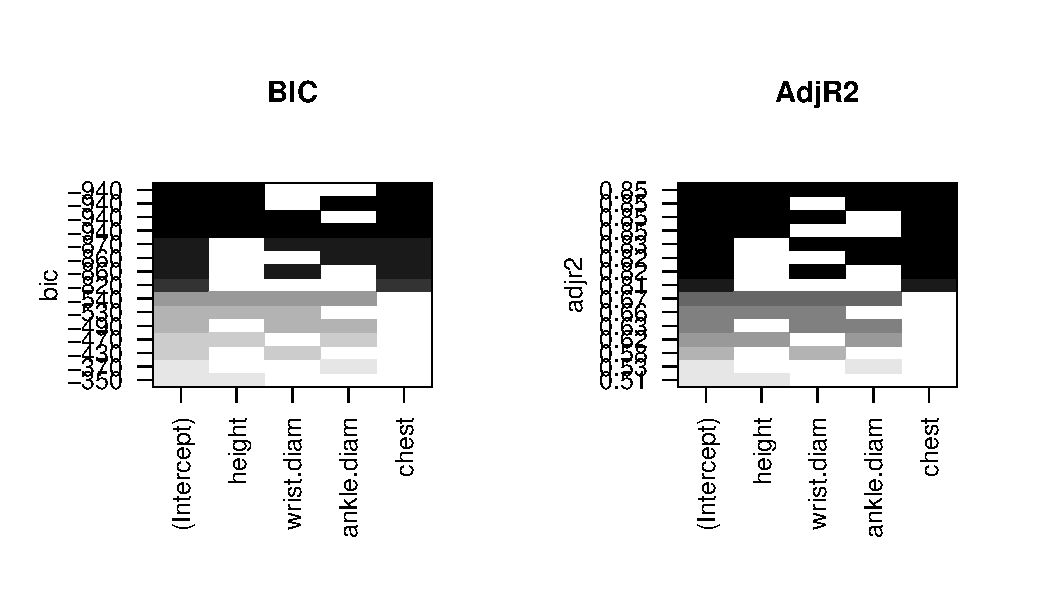
\includegraphics[width=\maxwidth]{figure/leap} 

\end{knitrout}

}
\end{frame}


%------------------------------------------------

\begin{frame}{Summary (Emily)}

{\fontsize{0.275cm}{1em}\selectfont 
\caption{Criteria Summary for each model}\\

\begin{center}
\begin{tabular}{|r|c|c|c|c|r|}
  \hline
MLR\# & AIC & BIC & PRESS & Adjusted $R^2$ & Method \\ 
  \hline
all & 2216 & 2326 & 2384 & 0.9753 & \text{all variables  from dataset used} \\ \hline
i & 2970 & 3004 & 10405 & 0.8869 & \text{suggested by paper} \\ \hline
1 & 2256 & 2319 & 2560 & 0.9727 & \text{suggested by paper}\\ \hline
2 & 2402 & 2441 & 3408 & 0.9632 & \text{my model}\\ \hline
3 & 2206 & 2282 & 2329 & 0.9754 & \text{stepAIC} \\ \hline
4 & 2195 & \textcolor{blue}{2271} & \textcolor{blue}{2281} & \textcolor{blue}{0.9759} & \text{stepAIC and adjustments} \\ \hline
5 & 2207 & 2292 & 2335 & 0.9755 &\text{leaps (adj} R^2) \\ \hline
6 & \textcolor{red}{2189} & 2278 & \textcolor{red}{2255} & \textcolor{red}{0.9764}  & \text{leaps(adj} R^2) \text{and adjustments}\\ \hline
7 & 2213 & 2272 & 2353 & 0.9749 & \text{leaps(BIC)} \\ \hline
8 & \textcolor{blue}{2205} & \textcolor{red}{2264} & 2316 & 0.9753 & \text{leaps(BIC) and adjustments}\\ \hline
\end{tabular}\\
\caption{\textit{\textcolor{red}{Red} corresponds to the best value for that criteria, \textcolor{blue}{blue} is the second best.}}
\end{center}

\begin{itemize}
\item Model Selection truely is an art form. 
\item R can mechanically run through steps, interactions, combinations, etc. 
\item R cannot subjectively look at the variables to determine the absolute best model. 
\item To acheive the model of ``best" fit, it is best to utilize a combination of R functions, criteria methods, and your own adjustments/ intuition.
\end{itemize}
}

\end{frame}

%------------------------------------------------

\subsection{Logistic Regression and Ada-boosting}

%------------------------------------------------
\begin{frame}{Model Selection (Yiding)}
\begin{minipage}{\textwidth}
{\bf Logistic Model:}
     $logit(p_i)=\beta_0+\beta_1X_{i1}+...+\beta_mX_{im}$
\end{minipage}
     \begin{columns}[t] % contents are top vertically aligned
     \begin{column}[T]{5cm}
     {\fontsize{0.3cm}{1em}\selectfont
     {\bf Model selection criteria:}\\
     \begin{itemize}
     \item $AIC$\\
     =$nlog(RRS/n)+2(p+1)$\\
     in R: $step()$\\[2\baselineskip]
     \item $BIC$\\
    =$nlog(RSS/n)+(p+1)log(n)$\\
      \&\\
    Posterior Probability\\
    $=p(\theta \mid x)=\frac{p(x\mid\theta)p(\theta)}{p(x)}$\\
    in R: $BMA$ packages $bic.glm()$
    \end{itemize}
     }
     \end{column}
     \begin{column}[T]{7cm}
     \begin{table}[ht]
\centering
\resizebox{\textwidth}{!}{
\begin{tabular}{rlc}
  & {\bf AIC} criteria model selection&\\
  \hline
  Step \# & Model & AIC \\ 
  \hline
  1 & $logi$(SEX)=WT+CDM+CDP+BDM+WR+ANK+HT+AGE+SHD+NAV+HIP & 110.35\\
  2 & $logi$(SEX)=WT+CDP+BDM+WR+ANK+HT+AGE+SHD+NAV+HIP & 108.36\\
  3 & $logi$(SEX)=WT+CDP+BDM+WR+HT+AGE+SHD+NAV+HIP & 106.45\\
  4 & $logi$(SEX)=CDP+BDM+WR+HT+AGE+SHD+NAV+HIP & 104.55\\
  5 & $logi$(SEX)=CDP+WR+HT+AGE+SHD+NAV+HIP & 102.69\\
  6 & $logi$(SEX)=CDP+WR+HT+AGE+SHD+HIP & 101.05\\
   \hline
\end{tabular}
}
\end{table}


\begin{table}[ht]
\centering
\resizebox{0.89\textwidth}{!}{
\begin{tabular}{rlrc}
  & {\bf BIC} criteria model selection& &\\
  \hline
  Model \# & Model & BIC & Posterior prob\\ 
  \hline
  1 & $logi$(SEX)=WR+HT+SHD+HIP & -3033 & 0.453\\
  2 & $logi$(SEX)=WR+HT+AGE+SHD+HIP & -3031 & 0.157\\
  3 & $logi$(SEX)=CDP+WR+HT+AGE+SHD+HIP & -3031 & 0.151\\
  4 & $logi$(SEX)=WR+HT+SHD+NAV+HIP & -3031 & 0.142\\
  5 & $logi$(SEX)=WR+HT+SHD+HIP & -3029 & 0.047\\
   \hline
\end{tabular}
}
\end{table}
     \end{column}

     \end{columns}
\end{frame}
%------------------------------------------------

\begin{frame}{Check the Goodness of Model (Yiding)}
\begin{columns}[t]
\begin{column}[t]{5cm}
{\fontsize{0.3cm}{1em}\selectfont
\begin{itemize}
\item \textbf{Linearity}\\
\underline{Residuals vs Fitted Values}\\
Pearson residuals:\\
$r_i=\frac{y_i-\hat{\mu}_i}{\sqrt{\hat{V}(y_i)}}=\frac{y_i-n_i\hat{\pi}_i}{\sqrt{n_i\hat{\pi}_i(1-\hat{\pi}_i)}}$\\[3\baselineskip]

\item{\textbf{Predictive ability}}\\
\underline{ROC curve}:\\
sensitivity $vs$ 1-specificity\\
\underline{Somer's rank correlation}:\\
$D_{xy}=2(c-0.5)$\\
$c$ is the area under the ROC curve.\\[1\baselineskip]
$Hmisc$ package: $somers2()$
\end{itemize}

}
\end{column}

\begin{column}[t]{7cm}
\begin{knitrout}
\definecolor{shadecolor}{rgb}{0.969, 0.969, 0.969}\color{fgcolor}
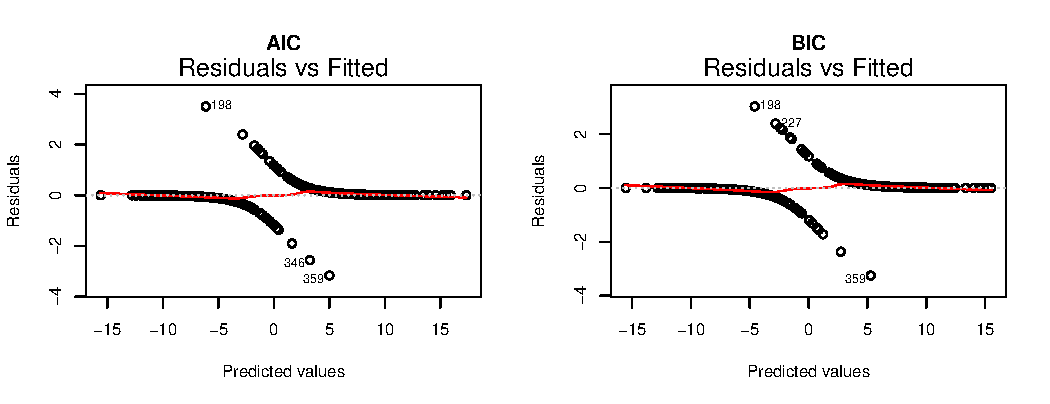
\includegraphics[width=\maxwidth]{figure/AIC_BIC_RESIDUALS} 

\end{knitrout}


\begin{knitrout}
\definecolor{shadecolor}{rgb}{0.969, 0.969, 0.969}\color{fgcolor}
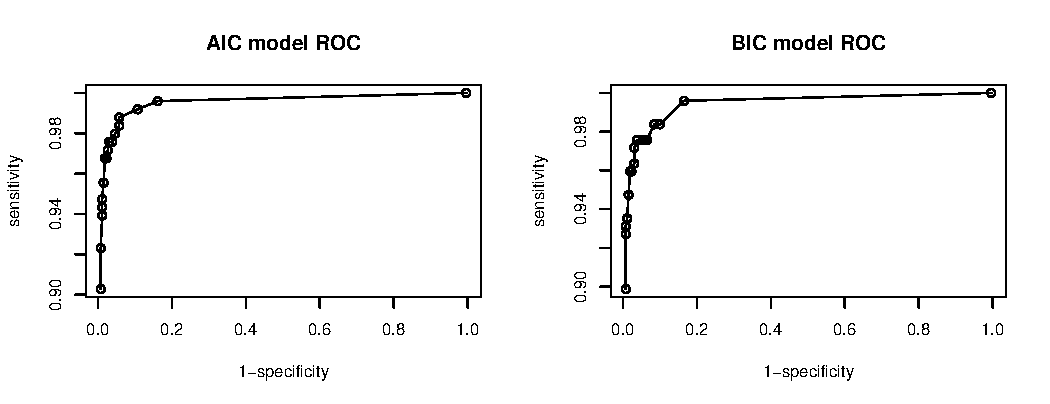
\includegraphics[width=\maxwidth]{figure/prdict_ability} 

\end{knitrout}


\begin{table}[ht]
\centering
\resizebox{0.6\textwidth}{!}{
\begin{tabular}{ccc}
  \hline
  Model  & Area ROC curve & Somers' $D_{xy}$\\ 
  \hline
  AIC & 0.9944721 & 0.9889443\\
  BIC & 0.9941607 & 0.9883214\\
   \hline
\end{tabular}
}
\end{table}
\end{column}
\end{columns}

\end{frame}
%------------------------------------------------

\begin{frame}{Ada-boosting (Yiding)}
\begin{columns}[T]
\begin{column}[t]{5cm}
{\fontsize{0.2cm}{1em}\selectfont
\textbf{Algorithem}:\\
Given: $(x_1,y_1),...,(x_m,y_m)$ where $x_i \in X, y_i \in Y=\{-1,+1\}$ Initialize $D_1(i)=1/m$.\\
For $t=1,...,T$:\\
$\bullet$ Train weak learner using distribution $D_t$.\\
$\bullet$ Get weak hypothesis $h_t : X \rightarrow \{-1,+1\}$ with error $\epsilon_t=Pr_{i\sim D_t}\left[ h_t(x_i)\ne y_i \right]$\\
$\bullet$ Choose $\alpha_t=\frac{1}{2}ln\left(\frac{1-\epsilon_t}{\epsilon_t}\right)$\\
$\bullet$ Update:\\
$$
D_{t+1}(i)=\frac{D_t(i)}{Z_t}\times
\left\{ 
\begin{matrix}
e^{-\alpha_t} & \mbox{if $h_t(x_i)=y_i$}\\
e^{\alpha_t} & \mbox{if $h_t(x_i)\ne y_i$}
\end{matrix}
\right.
$$\\
$=\frac{D_i(i)exp(\alpha_t y_i h_t(x_i))}{Z_t}$ \\
Final hypothesis: $H(x)=sign\left(\sum_{t=1}^{T}\alpha_t h_t(x)\right)$

}
\end{column}

\begin{column}[t]{7cm}
\begin{knitrout}
\definecolor{shadecolor}{rgb}{0.969, 0.969, 0.969}\color{fgcolor}
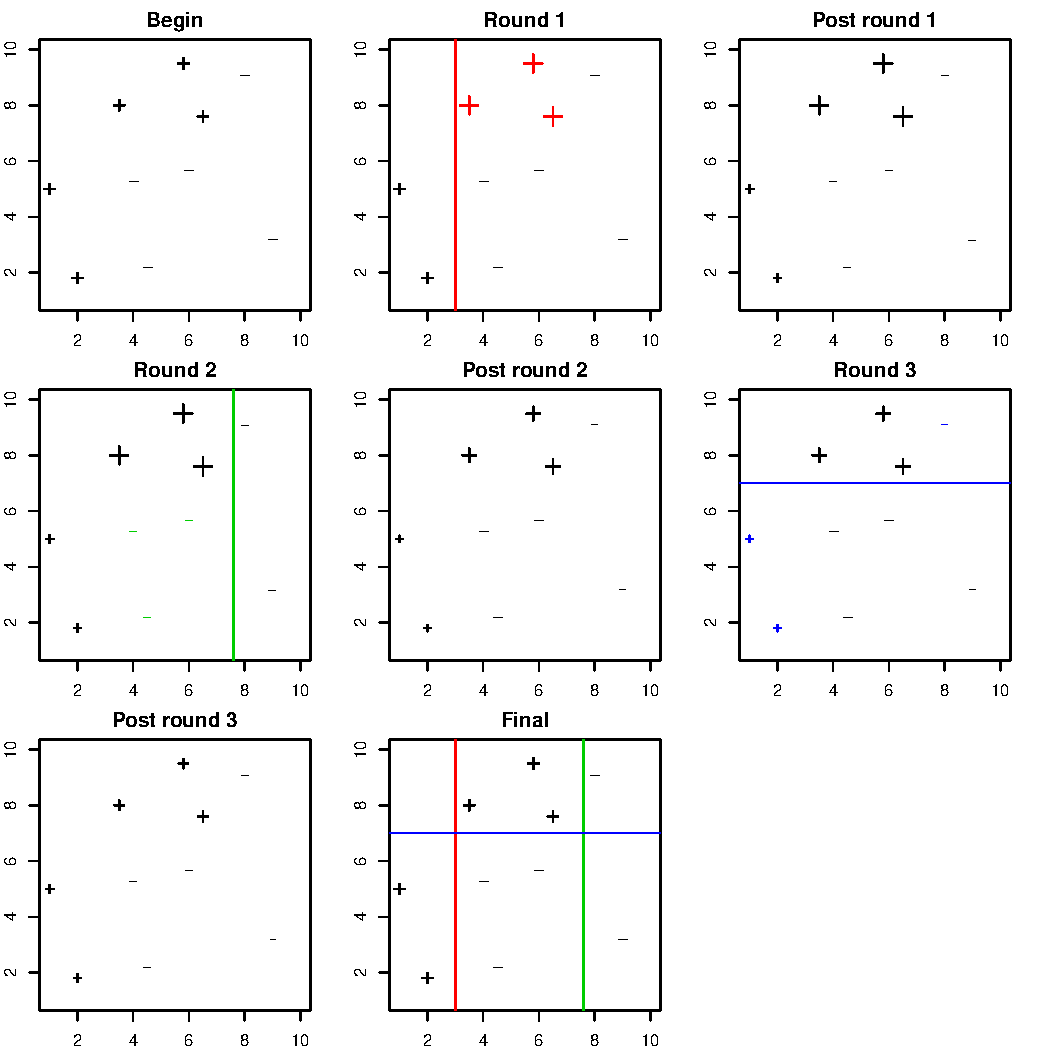
\includegraphics[width=\maxwidth]{figure/unnamed-chunk-2} 

\end{knitrout}


\end{column}

\end{columns}
\end{frame}
%------------------------------------------------
\begin{frame}{Logistic Regression vs Ada-boosting (Yiding)}
\begin{columns}[t]
\begin{column}[t]{4cm}
{\fontsize{0.3cm}{1em}\selectfont
\textbf{Logistic Regression}\\
Predictive ability depends on \underline{cutoff point}\\
}
\begin{table}[ht]
\centering
\resizebox{0.7\textwidth}{!}{
\begin{tabular}{ccc}
  \hline
  Cutoff point  & Sensitivity & Specificity\\ 
  \hline
  0.00 & 1.000 & 0.004\\
  0.05 & 0.996 & 0.838\\
  0.10 & 0.992 & 0.892\\
  0.15 & 0.988 & 0.942\\
  0.20 & 0.984 & 0.954\\
  ... & ...    & ... \\
  0.85 & 0.923 & 0.992\\
  0.90 & 0.903 & 0.992\\
   \hline
\end{tabular}
}
\end{table}


\end{column}
\begin{column}[t]{8cm}
{\fontsize{0.3cm}{1em}\selectfont
\textbf{Ada-boosting}\\
Predictive ability depends on \underline{variables}\\
}
\begin{table}[ht]
\centering
\resizebox{\textwidth}{!}{
\begin{tabular}{ccccc}
  \hline
  Round $\#$  & Original data & AIC data & BIC data\\
       & Sensitiviy; Specificity; Accuracy & Sensitiviy; Specificity; Accuracy & Sensitiviy; Specificity; Accuracy\\
  \hline
    1 & 0.975; 0.925; 0.949 & 0.967; 0.962; 0.965 & 0.967; 0.947; 0.957\\
    2 & 0.953; 0.936; 0.945 & 0.953; 0.920; 0.937 & 0.961; 0.936; 0.949\\
    3 & 0.949; 0.951; 0.949 & 0.954; 0.959; 0.957 & 0.954; 0.959; 0.957\\
    4 & 0.983; 0.932; 0.957 & 0.983; 0.955; 0.961 & 0.983; 0.962; 0.972\\
    5 & 0.983; 0.924; 0.953 & 0.983; 0.931; 0.957 & 0.983; 0.947; 0.965\\
    Average & 0.969; 0.934; 0.951 & 0.968; 0.945; 0.955 & 0.970; 0.950; 0.960\\
  \hline

\end{tabular}
}
\end{table}
\end{column}
\end{columns}


\begin{minipage}{\textwidth}
{\fontsize{0.3cm}{1em}\selectfont
\begin{columns}[t]


\begin{column}[t]{4cm}
\begin{itemize}
\item \textbf{Inference}\\
Logistic Regression $\surd$
\end{itemize}
\end{column}


\begin{column}[t]{8cm}
\begin{itemize}
\item \textbf{Prediction}\\
Ada-boosting $\surd$
\end{itemize}
\end{column}


\end{columns}
}
\end{minipage}


\end{frame}

%------------------------------------------------

\subsection{Regression Trees}

%------------------------------------------------

\begin{frame}{Differences between Males and Females (Liza)}
    \begin{columns}[t] % contents are top vertically aligned
     \begin{column}[T]{5cm} % each column can also be its own environment
   
\begin{itemize}
  \item Are there significant differences in the body measurements most useful for predicting weight in males and females?
  \item Is one regression formula appropriate for predicting weight for both genders?
  \item Can we use regression trees to help explore these questions?
\end{itemize}

\end{column}
\begin{column}[T]{7cm} % alternative top-align that's better for graphics


\begin{knitrout}
\definecolor{shadecolor}{rgb}{0.969, 0.969, 0.969}\color{fgcolor}
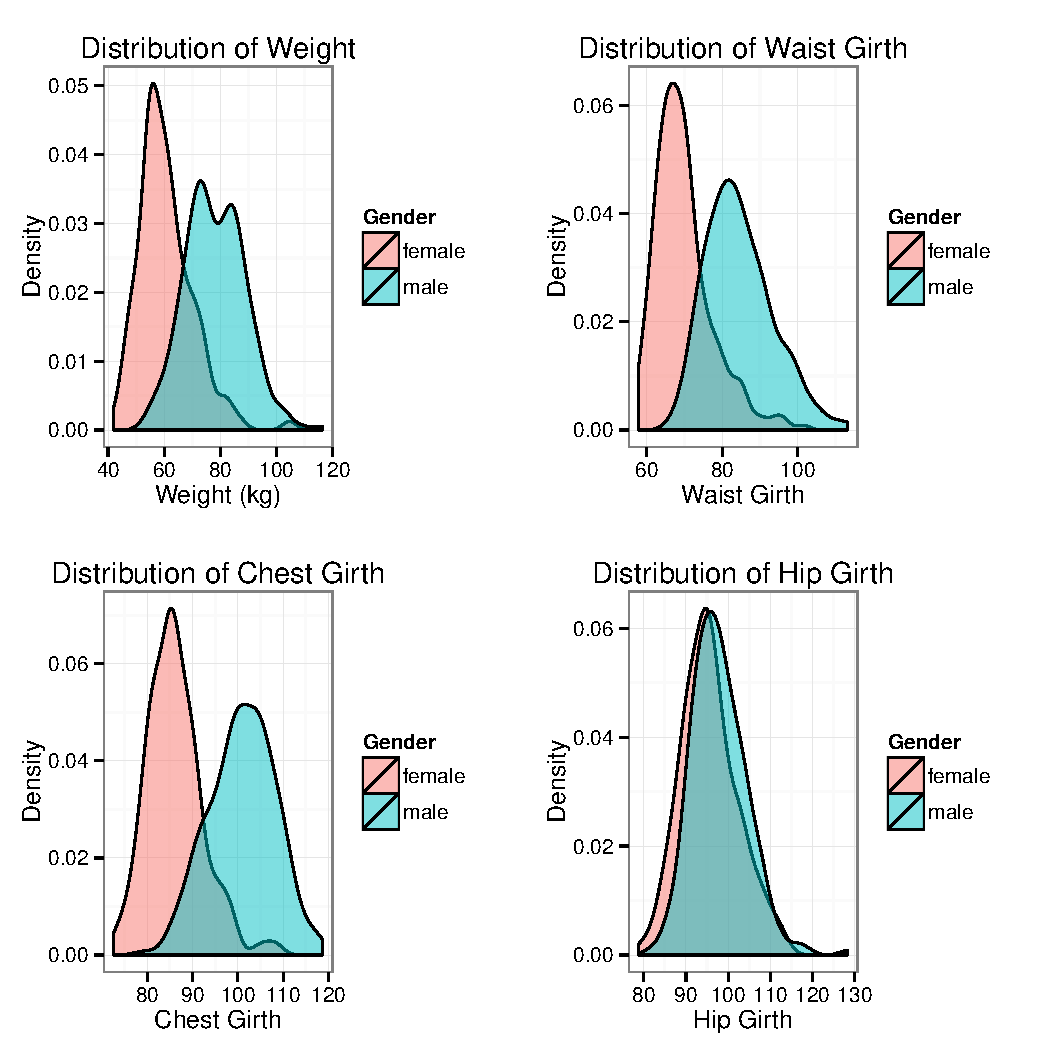
\includegraphics[width=\maxwidth]{figure/gender_plots} 

\end{knitrout}


     \end{column}
     \end{columns}
\end{frame}

%------------------------------------------------

\begin{frame}{Regression Trees (Liza)}

%this is the set-up for plotting regression trees



%here are the two regression trees. should be side-by-side with some text below.
\begin{knitrout}
\definecolor{shadecolor}{rgb}{0.969, 0.969, 0.969}\color{fgcolor}
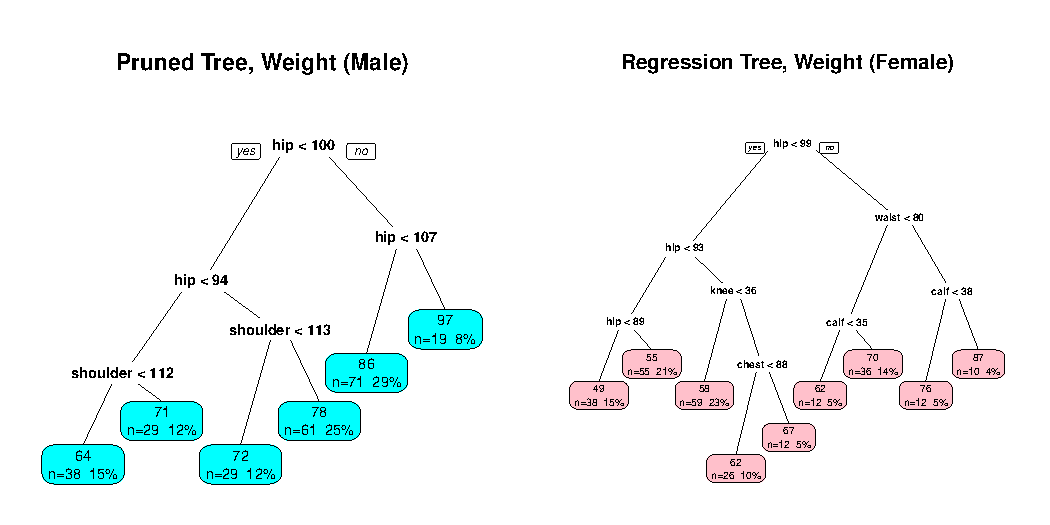
\includegraphics[width=\maxwidth]{figure/mf_plots} 

\end{knitrout}


\begin{itemize}
  \item Variables used in male tree: hip & shoulder girths
  \item Variable used in female tree: hip, knee, chest, waist and calf girths
\end{itemize}

\end{frame}

%------------------------------------------------

\begin{frame}{Conclusions (Liza)}

\begin{itemize}
    \item Regression trees are useful for exploring data and provide a useful alternative to parametric regression methods, though are not intended for making predictions.
  \item Results here suggest that separate models for males and females might be appropriate.
  \item Model fitting and selection exercises could test this hypothesis.
\end{itemize}

\end{frame}
%------------------------------------------------

\begin{frame}{Group Conclusions}
\begin{columns}[t]
\begin{column}[t]{4cm}

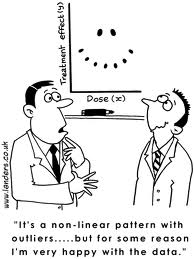
\includegraphics[width=\textwidth]{happy}

\end{column}


\begin{column}[t]{8cm}
What have we learned? 

\begin{itemize}
  \item Always check your assumptions, even low influence outliers can change your model fit
  \item With model selection, a combination of selection criteria, R functions and intuition are needed to create the model of ``best" fit. 
  \item Inference choose Logistic Regression; prediction choose Ada-boosting.
  \item Regression trees are a powerful, yet simple, non-parametric method for exploring data.
  \item If time allowed, a combination of methods shown may produce and even better fitting model.
\end{itemize}
\end{column}
\end{columns}
\end{frame}

%----------------------------------------------------------------------------------------

\end{document} 
